%!TEX program = xelatex
% 完整编译: xelatex -> bibtex -> xelatex -> xelatex
\documentclass[lang=cn,11pt,a4paper]{elegantpaper}

\title{汇编课程大作业:汇编游戏INVERSUS}
\author{林欣涛 \\ 软件01 \\ 2020012356 \and 杜家锟 \\ 软件01 \\ 2020010795 \and 朱思漠 \\ 软件92 \\ 2018012209}

\date{}

\usepackage{listings}


\begin{document}

\maketitle

\section{选题说明}

在本次课程作业中,我们利用汇编语言实现了Inversus游戏。本游戏取材自switch游戏Inversus Deluxe,其在PC和PS端均有发布,是一个有一定热度的游戏。而该游戏的实现逻辑没有任何参考样例,我们对规则的实现基本上是考虑到均衡性和可玩性进行原创的,在原创规则集上完成了大作业的内容。

\begin{figure}[htbp]
    \centering
    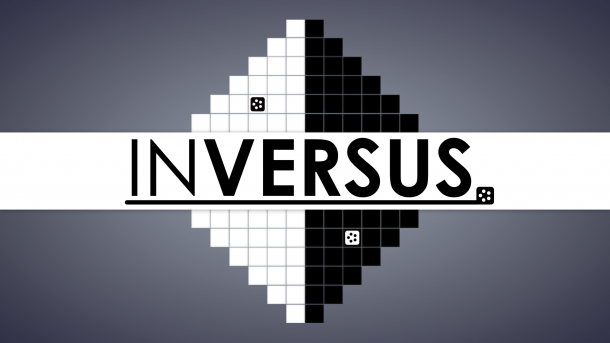
\includegraphics[width=0.5\linewidth]{img/title.jpg}
    \caption{Inversus游戏的宣传图}
    \label{F1}
\end{figure}

Inversus趣味性强,适合两人对战,核心规则为:每个玩家只能在与自己颜色相反的区域内移动;玩家通过射击子弹可以扩展领地;子弹射中对手获得胜利(另有子弹对撞抵消、子弹冷却等补充规则)。许多规则简洁明了的游戏都有着相当讲究的策略,Inversus也是如此,领地交错和射速约束提供了局面发展的复杂性,考验玩家的技巧和策略。玩家需要使用子弹扩展领地,保证运动范围和躲避空间,伺机将对手压缩在比较狭小的区域内,最终击中对手取得胜利。

\begin{figure}[htbp]
    \centering
    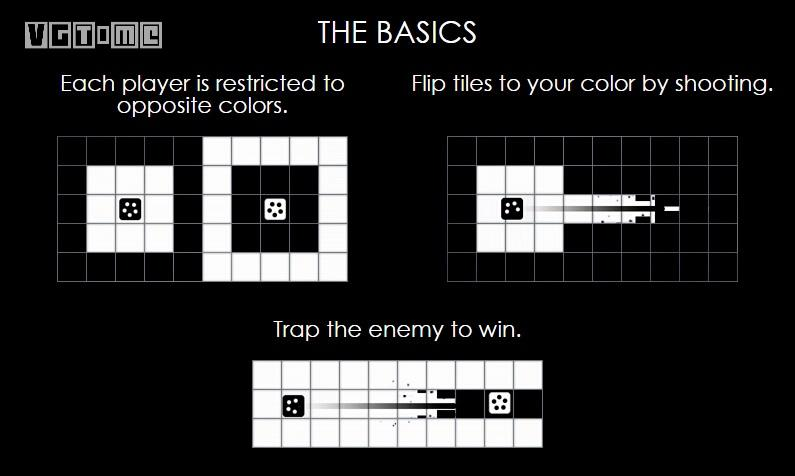
\includegraphics[width=0.5\linewidth]{img/inversus.jpg}
    \caption{Inversus游戏的大致规则示意}
    \label{F2}
\end{figure}
\clearpage

\section{开发环境}
\noindent \textbf{操作系统}:Windows 10。

\noindent \textbf{集成开发环境}:Visual Studio(2012、2019与2022三个版本均可运行)。

\noindent \textbf{运行方法}:安装MASM32,导入附加依赖项Irvine32,完成汇编环境配置。在Visual Studio中就可以使用Debug或Release模式运行并生成.exe文件。

\noindent \textbf{文件结构说明}:
\begin{itemize}
    \item \verb|src|文件夹下存放代码文件,包括\verb|.asm|汇编文件与资源文件。
    \item \verb|exe|文件夹下存放可执行文件,包括\verb|.exe|可执行文件以及运行说明\verb|readme.txt|。
    \item \verb|doc|文件夹下存放说明文件。
\end{itemize}

\section{实现原理}
\subsection{原理总述}

我们使用汇编语言,调用Win32相关API实现图形界面绘制、绘图、键盘控制、音效播放、定时触发等用户交互功能,从而完成两个玩家对战的Inversus游戏。

\subsection{窗口绘制}

图形界面的绘制主要参考了\href{https://learn.microsoft.com/zh-cn/windows/win32/api/}{Win32 API官方文档},概括而言,我们使用了两种实现方式:控制画刷直接绘制色块,以及在界面上显示图片资源。

对于选关界面这种需要查看所有关卡大体情况的界面,具体的地图使用画刷绘制非常繁琐,所以我们通过\verb|BitBlt|函数直接插入各个关卡地图简图的方式实现。

对于其他界面,包括菜单界面、游戏界面、帮助界面、自定义颜色界面,我们都选择使用画刷绘制实现。这种实现方式使得我们的程序具有极大的可扩展性(这一点在创新点部分会详细描述)。

为了解决中期时未能解决的“屏幕闪烁”问题,我们采取了先将所有需要绘制的元素绘制到一张”布局页面”句柄上,最后再将“布局页面”整个绘制到屏幕上的方式,这类似于图形学渲染中的帧缓冲(framebuffer)方法。这样既减少了在屏幕上重新绘制的次数,使得屏幕的显示更加稳定,也解决了此前出现的屏幕闪烁问题。

\subsection{按键响应}

为了实现按键事件的响应与处理,我们在消息循环当中识别\verb|wm_keydown|和\verb|wm_keyup|两类事件消息,随后控制跳转,执行对应的消息处理过程。在\verb|keydownmessage|的实现过程中,我们通过查找资料获取键盘按键字符码,与按键信息的下一位键盘信息进行比较,若比对成功则标记该键的状态为1,否则直接结束按键消息;同样,在\verb|keyupmessage|中,通过与按键信息的下一位键盘信息进行比较,若比对成功则标记该键的状态为0,否则直接结束按键消息。

\subsection{定时器信息}

定时器的设置需要保证在窗口创建的时候就开始设置,而在窗口关闭时候结束掉。通过定时器的回调函数,我们实现了每30ms更新一次场面上的方块位置信息、子弹位置信息和地图信息等数据,并调用重绘函数重新绘制黑白角色、子弹位置与地图画面,代码略如下。

\lstset{
    language={[x86masm]Assembler},
    basicstyle=\tt\small,
    keywordstyle=\color{purple}\bfseries,
    identifierstyle=\color{brown!80!black},
    commentstyle=\color{gray},
    showstringspaces=false,
    numbers=left,
}
\begin{lstlisting}[title=代码1:定时器]
INVOKE SetTimer, hWnd, 1, 30, NULL    ; 开启定时器
cmp eax, WM_TIMER      ; 接受定时器消息
je TimerMessage        ; 设计了一个定时器执行函数
INVOKE KillTimer, hWnd, 1    ; 关闭定时器
\end{lstlisting}

\subsection{方块移动}

为了实现方块(角色)在地图上的\textbf{平滑移动},在定时器回调函数中,我们逐一判断每一个按键的状态是否为1(代表按键按下),如果按下就修改其数值,没有按下就跳过。这样紧随其后的窗口重绘函数就会调用画图函数重新绘制黑白主角的位置,从而实现平滑移动;效果上讲,同时按键的持续时间越长,移动的距离越远,并且角色不会出现瞬间移动,而是平滑过渡到新位置。

\subsection{子弹射击}

我们将子弹射击与后续判定两个过程进行解耦,分为下面两个函数:

\begin{itemize}
    \item \verb|emitBullet|函数在攻击键被按下时调用,它的作用是向地图中加入一发子弹,其位置、方向、颜色均取决于发射它的角色当前的状态。同时,程序将会新创建一个线程用来播放音效。
    \item \verb|updateBullets|则负责对场上所有子弹的状态进行结算,更新元数据并重绘画面,包括且不限于更新子弹位置、双方子弹对冲抵消、子弹射出地图后清除、子弹导致的路径变色、路径变色导致的敌方角色死亡。\verb|updateBullets|在定时器函数中被调用,使得子弹的更新也是平滑进行的。
    \item 值得着重指出的是,我们使用\textbf{多线程异步播放}射击音效,射击音效紧跟射击操作,不会因冲突而滞后或中断,游戏氛围更加紧张刺激。
\end{itemize}

此外,子弹的\textbf{冷却功能}借助计时器函数实现,每当一个计时器周期(30ms)到来时,计数器将加一。当计数器的值达到50时(即1.5秒后),计数器将清零,并令子弹数加一。这个功能保证了子弹不能无限发射,加强了游戏的策略性。


\subsection{游戏暂停}

我们为游戏设计了暂停功能。在游戏过程中,如果Esc键被按下,将会使得游戏标志位\verb|statusFlag|置为3,代表了游戏当前处于暂停状态。而计时器函数在执行前将检测这个标志位,当\verb|statusFlag|值为3时,计时器函数直接退出,不做任何事。此时所有的角色控制操作都无法响应,依赖于计时器调用的子弹更新函数\verb|updateBullets|也不再运行,从而实现了暂停的效果。而按下C键会继续游戏,按下Q键则退出本局游戏,这些我们在界面上都设计了用户提示信息,方便用户交互。

\subsection{颜色自定义}

为了增强\textbf{游戏的自由度},我们设计了自定义颜色的功能,玩家可以个性化设置角色专属颜色和背景颜色。为了实现颜色自定义功能,我们修改了角色显示的方式。我们最初的实现是将角色的图片直接画在屏幕上,但这样的方法难以扩展,如果希望改变角色专属颜色,就必须重新找一张图片进行替换。除此之外,20张资源图片的载入也会导致程序的体积过于臃肿。于是,我们选择用画刷绘制角色的方式代替使用图片绘制角色,这样只需要改变画刷使用的颜色句柄,即可实现角色颜色切换。这样的方式也方便了开发中的功能扩展,例如,刚做出来此功能时,选取的20种颜色中有两对颜色较为接近,如果同时被选择则容易混淆。但是修改起来极为方便,只需修改\verb|const.inc|中的颜色数组,就可快速地改变颜色,省去了重新找资源文件的过程。

\begin{figure}[htbp]
    \centering
    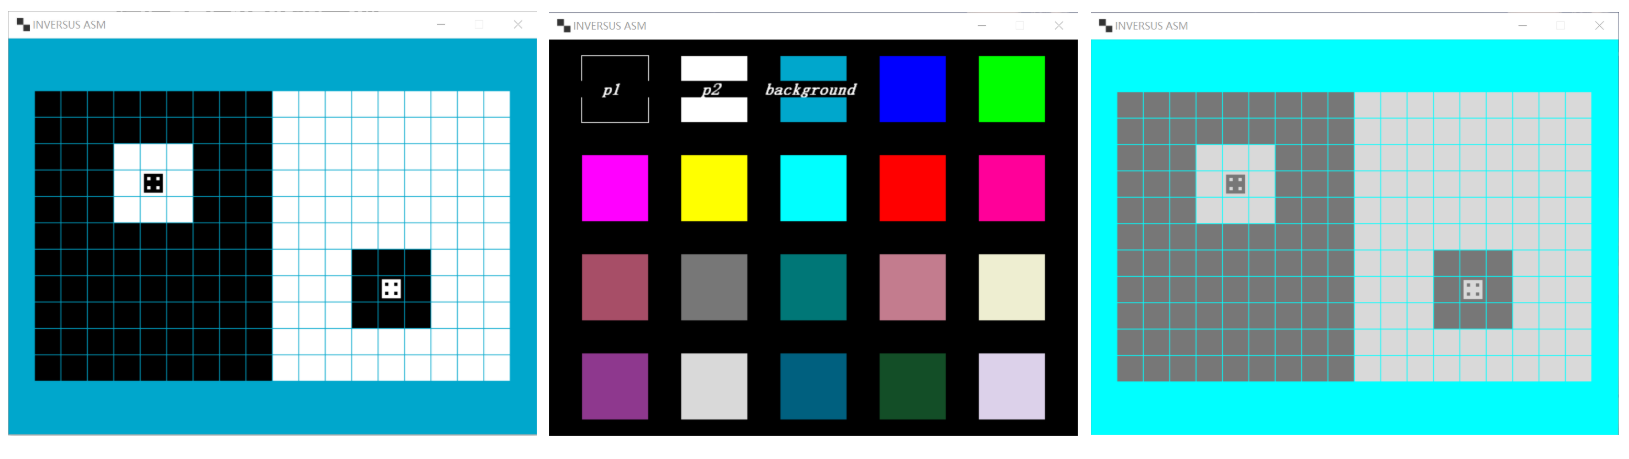
\includegraphics[width=0.95\linewidth]{img/color.png}
    \caption{角色颜色自定义过程示意}
    \label{F3}
\end{figure}

\subsection{帮助信息}

作为一款游戏,我们有职责在游戏内解释交互逻辑、操作方法和对战方式。为此,我们设计了Help模块对应的帮助界面,通过界面内绘制帮助信息的方式,为用户提供了交互模式介绍。此外,在菜单选择中,我们也为用户提示了选择、切换方式;在游戏的暂停界面,我们也为用户介绍了恢复和退出的方法。充分且恰到好处的帮助信息是保障用户交互体验的不二法门。

\subsection{内存保护}

这个部分主要是在接收到程序关闭信号的时候,使用\verb|delete|操作删除在\verb|createwindows|时创建的所有句柄,防止由于句柄创建过多导致的内存泄漏,有力保障内存安全,消除了对程序\textbf{稳定性}的威胁。

\subsection{游戏名呼吸灯设计}

在进入游戏的界面,我们为游戏名称设计了\textbf{呼吸灯效果},通过巧妙设计颜色的起始、终止数值与颜色间隔,实现颜色的缓慢变化。主要设计代码如下:

\begin{lstlisting}[title=代码2:游戏名呼吸灯]
INVOKE SelectObject, hdcMempage, font_100
mov eax, judgeup
cmp judgeup, 0
je @colordown
	add titlecolor, 00030302h
	cmp titlecolor, 00ffffAAh
	jne @drawtitle
	mov eax, 0
	mov judgeup, eax
@colordown:
	sub titlecolor, 00030302h
	cmp titlecolor, 00696946h
	jne @drawtitle
	mov eax, 1
	mov judgeup, eax
@drawtitle:
	INVOKE SetTextColor, hdcMempage, titlecolor
	INVOKE SelectObject, hdcMempage, font_100
	INVOKE TextOutA, hdcMempage, 100, 30, offset gamename, 8
	INVOKE SelectObject, hdcMempage, font_50
	INVOKE TextOutA, hdcMempage, 270, 130, offset gamebanben, 3
\end{lstlisting}

\section{难点和创新点}

\subsection{难点一:图形界面搭建与完善}

我们的项目是一款游戏,游戏最重要的就是游戏体验,而用户最直观的游戏体验就是\textbf{图形界面}。因此在我们项目的初期,图形界面的绘制就是我们小组攻坚的重中之重。起初,由于我们对Win32绘图相关API尚不熟悉,我们连一个基本的图片绘制都成问题,并且踩了一些比较冷门的坑。后来,经过几天的摸索,我们成功显示了第一张图片,之后我们才将基本的游戏界面绘制出来。

然而对我们来说,这还不够。当时我们只能实现“能看”,但用户体验不佳——游戏界面的显示总是在不停地闪烁。我们对这个问题感到非常困惑,尝试了许多方案都没有解决。于是,我们仔细重新研究了一下Win32绘图相关API,并对绘图函数进行了重构,在重构后我们找到了解决问题的方法:增加了一个“\textbf{布局页面}”句柄,先将所有需要绘制的元素绘制到它上面,在所有元素都绘制完之后,再将它整个绘制到屏幕上,类似于图形学渲染中的帧缓冲。这样的绘制方式,减少了直接在屏幕上绘制的次数,屏幕闪烁的问题迎刃而解,玩家的游戏体验大大提高。

\subsection{难点二:汇编项目架构与项目管理}

由于我们使用的是汇编语言这种底层的语言,我们在\textbf{项目架构}搭建方面遇到许多细节问题,我们在走了一些弯路之后解决了架构问题。而在项目管理方面,由于汇编缺少面向对象的能力,不加管理的汇编代码很容易出现难以继续开发的“屎山”,被迫变成“只读”代码,不利于迭代开发。这在项目中期前后给我们带来了不少困扰。

中期以后,我们进行了两轮\textbf{代码重构},充分利用汇编语言进行面向过程的编程,使用更具意义、更明确的变量命名规范、添加大量可读注释,完善事件循环与过程逻辑,合理划分各方法的功能边界。我们还利用了软件工程课上学习的项目管理方案,利用git进行版本控制\href{https://github.com/linxt20/-INVERSUS_masm}{Github项目仓库},在代码重构的基础上进行了几轮\textbf{迭代开发},既保证项目进度,又保证项目的代码质量和可读性、可扩展性。

\subsection{创新点一:角色的平滑移动控制与打击感}

为了让玩家在玩我们的游戏时有更加流畅且爽快的游戏体验,我们在角色的移动和攻击上花了很大功夫。

首先是移动方面,最简单的实现方式莫过于“闪现式”的移动,但我们不满足于此,通过使用计时器实现对用户的按键输入高频检测,进而高频且低粒度地更新角色的位置,使得角色可以平滑移动,接近动画效果。

其次是攻击方面。我们同样使用计时器对发射的子弹位置进行更新,使得子弹的射击也趋于平滑。除此之外,为了能让玩家对“攻击”有一个直观的反馈,我们为每次攻击加上了音效。在开启音效的情况下,整场战斗将变得无比“带感”,游戏体验大大提高。

\subsection{创新点二:游戏设计与独特的攻击判断逻辑}

Inversus是一款射击游戏。射击游戏一般的攻击判定逻辑是把直接击中对方作为依据。但我们从玩家只能在与自己颜色相反的区域内移动这一基本设定出发,给出了新的\textbf{判定逻辑}——子弹并不直接对玩家造成伤害,子弹的唯一作用只是使得其路径变色。而一旦敌方角色有部分或全部像素处于变色的路径时,这意味着该角色所处的位置“不合法”,从而判定其被击败。

这样的判定规则,在具体表现上与传统的射击游戏存在差异:子弹无需“直接击中”目标也能造成击杀。此外,这样的判定规则,也与我们游戏的基本设定相辅相成:玩家只能在与自己反色的区域内移动。从而己方能移动的区域越大,则敌方能移动的区域越小。因此,通过子弹“开疆拓土”,在扩宽自己“活路”的同时限制敌方移动,是本游戏制胜的法宝。这样的设计有别于传统的射击游戏,使得我们的游戏独树一帜。Inversus的中文译名是“逆向”或者“逆转黑白”,其实也包含了这种意思。

\subsection{创新点三:可玩性、自由度与可扩展性强}

我们的游戏取材自switch游戏Inversus Deluxe,其可玩性和策略性已经在选题部分讲述了。我们没有直接照搬照抄,而是在其基础上做了自己的发挥。界面的高度个性化就是其中之一,我们为玩家提供了多达20种角色专属颜色,玩家可以从中挑选喜欢的颜色作为己方角色的专属颜色。另外,我们还支持设置游戏背景色。在此基础上,玩家拥有多达6840种配色方式,自由度非常丰富。除此之外,本游戏还留下了单人街机模式与双人联机模式的接口,配合上我们代码重构的成果,给游戏的未来发展留下了更多的可能。

\section{与中期相比的进展}

相比于中期,我们的项目完成了质的飞跃。中期我们实现了游戏的基本架构搭建,例如计时器函数、仅绘制了开始、模式选择和第一关卡三个页面、角色平滑移动(不包括位置合法性判断)、仅有2个菜单栏切换。当时的项目尚处于起步阶段。与之相比,我们的终稿有了全面的提高。我们增加的功能如下:


\begin{enumerate}
    \item 使用画刷绘图代替大体积图片的显示,最后程序大小从原来的30+MB缩减到不足2MB,缩小了游戏文件的占用空间。
    \item 包含位置合法性的角色移动,并且支持平滑移动。
    \item 详细的帮助界面和页面提示、按键提示等提示信息。
    \item 新增多个游戏地图以及地图选择界面,大大提高游戏的多样性。
    \item 子弹发射操作、移动逻辑、位置合法判定,实现了子弹的结算,包括角色胜负判断、地图变色动画以及子弹对撞相消等多种功能。
    \item 设置了子弹的恢复冷却cd,在角色上显示子弹储备量,让玩家对于当前游戏局势有一个清晰的了解。
    \item 使用多线程异步播放射击音效,实现射击音效紧跟射击操作。
    \item 完善进入地图的数据初始化,游戏的暂停、退出、继续等设计,胜利判定与胜利界面设计。
    \item 设计了颜色自定义功能,让用户能够自己选择角色以及背景色,增加游戏的趣味性和自由度。详细完善了在该界面的光标操作以及边界判断,操作手感丝滑。
    \item 关闭程序删除所有创建的句柄,保障内存安全,提高游戏稳定性。
    \item 游戏标题采用呼吸灯式的显示操作,提高界面的设计感。同时在字体和文字界面方面进行了重新设计,让游戏界面更加美观。
    \item 设计了自己独有的游戏图标(Icon)。
    \item 使用git管理代码(\href{https://github.com/linxt20/-INVERSUS_masm}{Github项目仓库}),兼容三种版本的Visual Studio开发环境,进行了代码重构,并且制定了合理的代码迭代计划。
\end{enumerate}
	
在代码结构方面,我们对中期前的代码进行了两轮重构,使得函数的逻辑更加清晰,这也为后续的扩展打好了基础。比如颜色自定义功能即是在重构后的绘图函数基础上搭建的。我们还为每个用到的库函数与变量添加了注释,为团队开发过程中小组成员间的交流和协助Debug铺平了道路,避免因不了解对方使用的变量与函数造成迷惑,从根本上杜绝了写出“屎山”代码的情况。另外,我们对代码风格也进行了修改,着重处理了重复、相似的代码段(例如冲突处理、光标的边界处理等),抽象为函数进行复用,并且将逻辑重叠的代码理顺、改写,大大提高了代码的可读性、复用性以及开发效率。


\section{小组分工}
林欣涛:按键识别与角色移动、绘制游戏界面与帮助界面、定时器处理函数、代码格式化。

杜家锟:游戏设计、菜单控制及绘制、子弹发射与相关判定、颜色自定义。

朱思漠:文档撰写、音效。

\end{document}